\documentclass[11pt]{article}

\usepackage[utf8]{inputenc} % Required for inputting international characters
\usepackage[T1]{fontenc} % Output font encoding for international characters
\usepackage{graphicx}
\usepackage{mathpazo} % Palatino font

\begin{document}

%----------------------------------------------------------------------------------------
%	TITLE PAGE
%----------------------------------------------------------------------------------------

\begin{titlepage} % Suppresses displaying the page number on the title page and the subsequent page counts as page 1
	\newcommand{\HRule}{\rule{\linewidth}{0.5mm}} % Defines a new command for horizontal lines, change thickness here
	
	\center % Centre everything on the page
	
	%------------------------------------------------
	%	Headings
	%------------------------------------------------
	
	\textsc{\LARGE Universität Hamburg}\\[1.5cm] % Main heading such as the name of your university/college
	
	\textsc{\Large Mashine Learning}\\[0.5cm] % Major heading such as course name
	
	\textsc{\large Exercise1}\\[0.5cm] % Minor heading such as course title
	
	%------------------------------------------------
	%	Title
	%------------------------------------------------
	
	\HRule\\[0.4cm]
	
	{\huge\bfseries Stochastic Gradient Descent}\\[0.4cm] % Title of your document
	
	\HRule\\[1.5cm]
	
	%------------------------------------------------
	%	Author(s)
	%------------------------------------------------
	
	\begin{minipage}{0.4\textwidth}
		\begin{flushleft}
			\large
			Benjamin Ostendorf\\
			Waijd Ghafoor% Your name
		\end{flushleft}
	\end{minipage}
	~
	\begin{minipage}{0.4\textwidth}
		\begin{flushright}
			\large
			Prof. Dr. Victor Emanuel de Atocha Uc Cetina\\
			Dr. Timo Baumann % Supervisor's name
		\end{flushright}
	\end{minipage}
	
	% If you don't want a supervisor, uncomment the two lines below and comment the code above
	%{\large\textit{Author}}\\
	%John \textsc{Smith} % Your name
	
	%------------------------------------------------
	%	Date
	%------------------------------------------------
	
	\vfill\vfill\vfill % Position the date 3/4 down the remaining page
	
	{\large\today} % Date, change the \today to a set date if you want to be precise
	
	%------------------------------------------------
	%	Logo
	%------------------------------------------------
	
	\vfill\vfill
	
\includegraphics[width=0.2\textwidth]{uni-siegel.png}\\[1cm] % Include a department/university logo - this will require the graphicx package
	 
	%----------------------------------------------------------------------------------------
	
	\vfill % Push the date up 1/4 of the remaining page
	
\end{titlepage}

%----------------------------------------------------------------------------------------
\section{Stochastic Gradient Descent}

\subsection{Implement in your favorite programming language the Stochastic Gradient Descent}

We decided to use Python version 3 for this exercise.

\subsection{Generate 100 artificial data points ($x_i$,$y_i$) where each $x_i$ is randomly generated from the interval [0,1] and $y_i = sin(2pi x_i) + e$. Here, e is a random noise value in the interval [-0.3,0.3]}


\begin{figure}[ht]
    \centering
    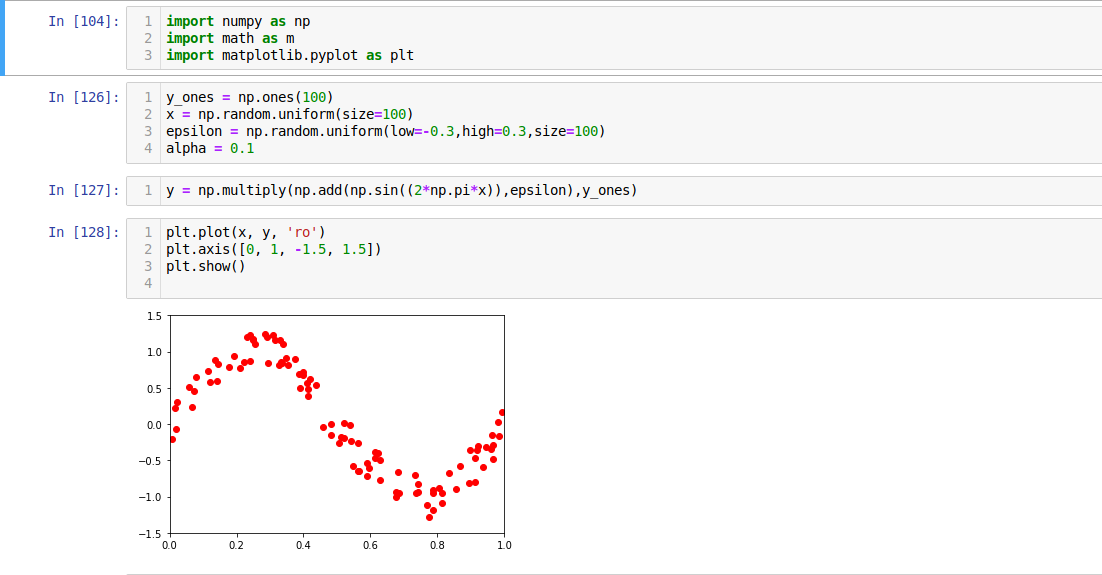
\includegraphics[width=\textwidth]{12.png}
    \caption{Plot of the sine function.}
    \label{12plot}
\end{figure}
In~\ref{12plot} it is shown how $x_i$ and $y_i$ are generated. We used the framework Numpy to generate the 100 random datapoints $x_i$ and $y_i$. After that we plotet $y_i$ and interesting is the Sinus shape. This was also our imagination, because we used the sin function with respect to the noise. Here we have to add that the random.uniform range includes the first intervall parameter (low), but excludes the second one (high). To create the original range, we decided to set high to the last possible float represention after 1.0.   

\subsection{Make youre initial learning rate constant  $\alpha = 0.1$, and train a polynomial model using your artificially created data. A polynomial model has the form $y = \Theta + \Theta \cdot x + \Theta \cdot x^{2} + \cdot \cdot \cdot + \Theta_M \cdot x^M$}

We implemenmted our polynomial Model and than we updated the $\Theta_i$ by our cost function:

\begin{align}
 J(\Theta) = \frac{1}{2} \sum_{i=1}^m[h_\theta(x^{(i)})-y^{(i)}}]^2
\end{align}
\begin{figure}[ht]
    \centering
    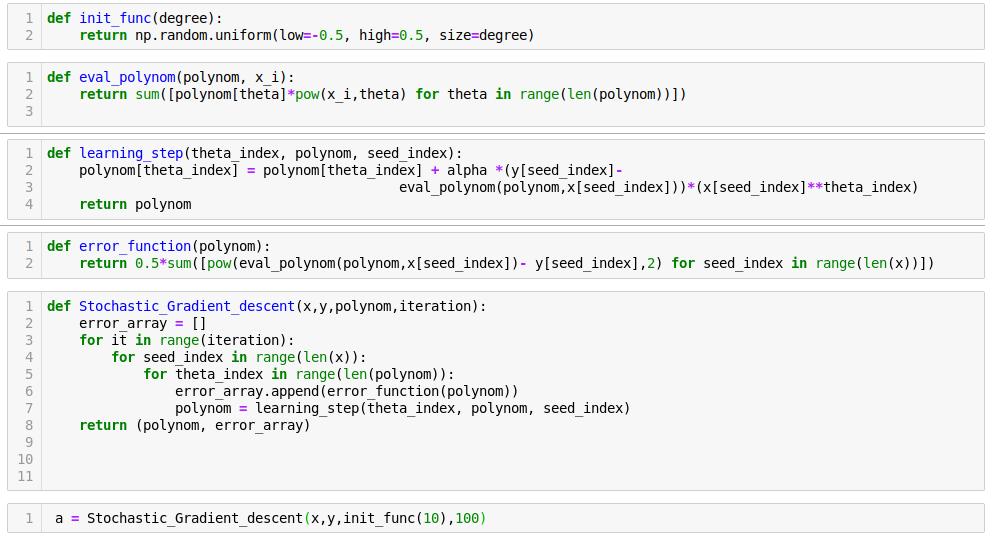
\includegraphics[width=\textwidth]{13.png}
    \caption{Plot of the implemented Stochastic greedy and descent}
    \label{13plot}
\end{figure}


\subsection{All initial $\Theta_i $ parameters are randomly generetad in the interval [-0.5,0.5]}
\begin{figure}[ht]
    \centering
    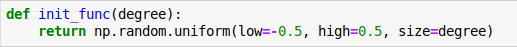
\includegraphics[width=\textwidth]{14.png}
    \caption{Function to decide the degree of the polynom}
    \label{14plot}
\end{figure}
In the Figure it is shown that the Thetas are generated randomly in the interval [-0.5,0.5]. Also the parameter of init-func returns the degree of the polynom.


\subsection{Try different $\alpha$ values to speed up the learning process}
High $\alpha$ returned a bad approximation of the sine function. Also values above 0.1 showed good values, but it is important to find the best iteration step. 

\begin{figure}[ht]
      \centering
      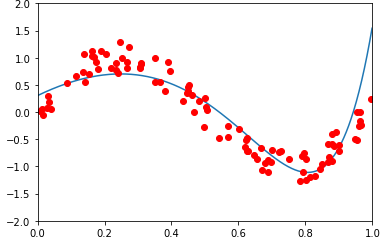
\includegraphics[width=0.3\textwidth]{15a.png}
      \caption{Plot for $alpha=0.2$.}
      \label{15aplot}
  \end{figure}

\begin{figure}[ht]
        \centering
        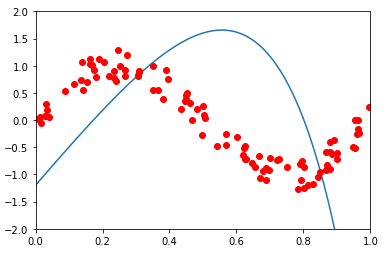
\includegraphics[width=0.3\textwidth]{15b.png}
        \caption{Plot for higher $alpha$.}
        \label{15bplot}
    \end{figure}

\begin{figure}[ht]
          \centering
          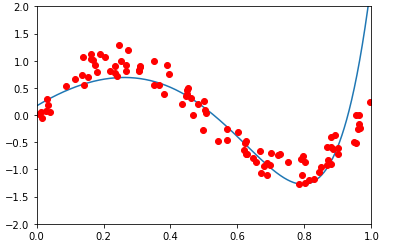
\includegraphics[width=0.3\textwidth]{15c.png}
          \caption{Plot for $alpha=0.3$.}
          \label{15bplot}
      \end{figure}

\subsection{Once you have found the best model, plot the graph containing the data points, the sine function, and the learned function.}

The following plots shows the results of our algorithmn. The higher the degree of the polynom the better results we achieved. But unfortunatly the runtime gets worse by higher degrees. If we remember correctly the degree of 3 by Prof. Dr. Victor Emanuel de Atocha Uc Cetina is in our example not sufficient to approximate the function closely enough. We have to add that we just iterated 100 times. 
\begin{figure}[ht]
    \centering
    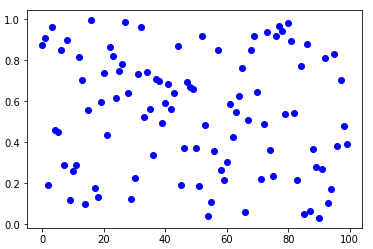
\includegraphics[width=0.3\textwidth]{16a.png}
    \caption{Plot of the random generated x values for the sin function}
    \label{16aplot}
\end{figure}
\begin{figure}[ht]
      \centering
      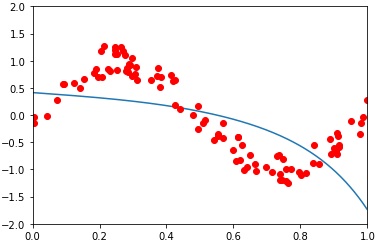
\includegraphics[width=0.3\textwidth]{initial.png}
      \caption{Plot of the initial function}
  \end{figure}

\begin{figure}[ht]
    \centering
    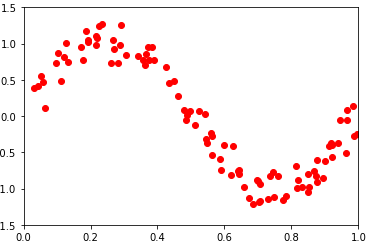
\includegraphics[width=0.3\textwidth]{16b.png}
    \caption{Plot of the sine function.}
    \label{16bplot}
\end{figure}
\begin{figure}[ht]
    \centering
    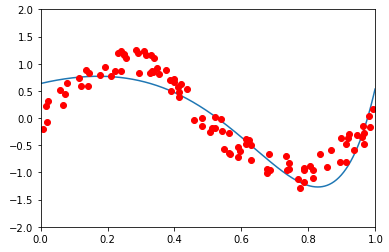
\includegraphics[width=0.3\textwidth]{16c.png}
    \caption{Plot of the learned function.}
    \label{16cplot}
\end{figure}

\newpage
\subsection{plot also the error curve.}
\begin{figure}[ht]
    \centering
    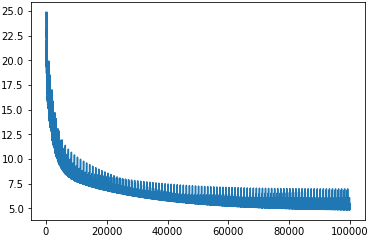
\includegraphics[width=0.3\textwidth]{17.png}
    \caption{Plot of the error curve.}
    \label{17plot}
\end{figure}

\subsection{Prepare a report containing your final model, your final $\alpha$ value, and ure graph}

Final Model where the Array[i] describes  the $\theta_i$
\begin{figure}[ht]
    \centering
    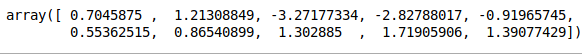
\includegraphics[width=\textwidth]{18.png}
    \caption{Plot of the Model with degree 9}
    \label{18plot}
\end{figure}

$alpha = 0.1$
The final graph is given:
\begin{figure}[ht]
      \centering
      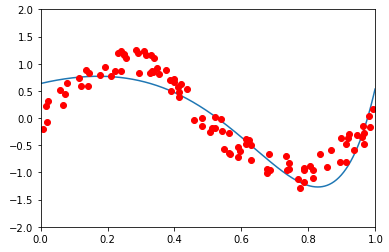
\includegraphics[width=0.3\textwidth]{16c.png}
      \caption{Plot of the final learned function.}
  \end{figure}

\end{document}

